\subsection{FP-based Approximate Indexing}
\label{sec:design:fp}

%\subsubsection{FP-based indexing}
%\label{sec:design:fp-basic}

Let us first explain how \ours{} manages a run in a tree using FP-based
indexing.  For each run $R_i$, logical blocks $x_i$ sorted by their LBAs are stored in
physically consecutive sectors $y_i$.  To map logical blocks $x_i$ to physical
sectors $y_i$, $R_i$ maintains a set of $<x_i,y_i>$ pairs in the memory: $R_i =
\{<x_0,y_0>,<x_{1},y_{1}>, ..., <x_{n-1},y_{n-1}>\}$, where $n$ is the number
of logical blocks (or sectors) in a run.  In \ours{}, $y_i$ increases by 1
monotonically, and thus it only needs to keep $x_i$ in $R_i$. Therefore,
$R_i$ can be rewritten as follows: $R_i = \{x_0,x_{1}, ..., x_{n-1}\}$.
Here, $x_i$ is a large integer number (\eg~32-bit for 16TB SSD) and 
increases as an SSD capacity grows. The FP-based indexing aims to reduce
the memory requirement by replacing $x_i$ with short fingerprints $FP_i$:
$R_i^{FP} = \{FP_0,FP_{1}, ..., FP_{n-1}\}$.

\begin{figure}[t]
\centering
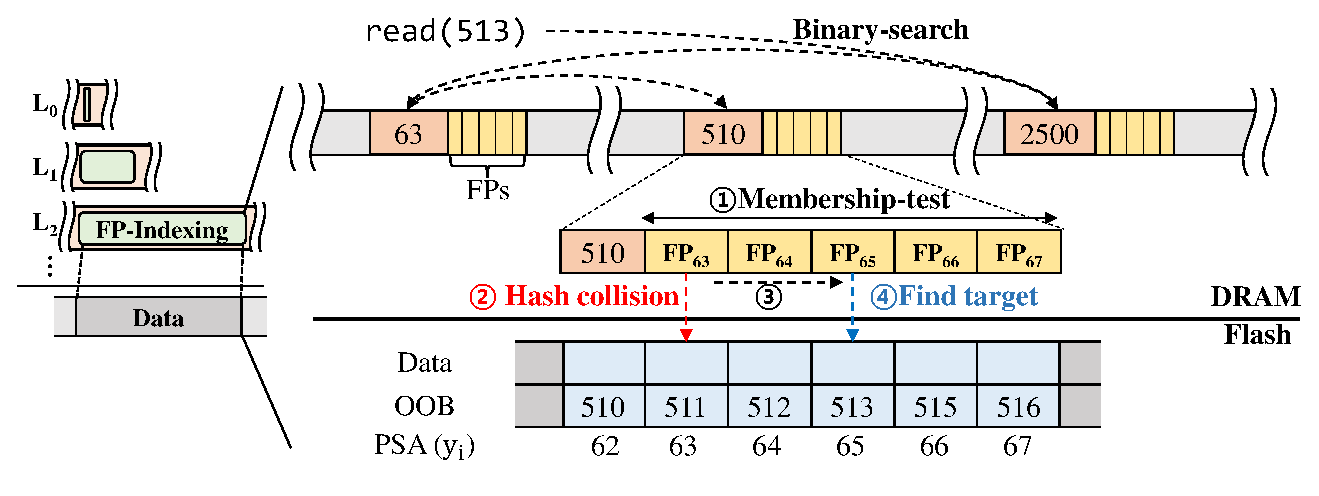
\includegraphics[width=0.45\textwidth]{figs/OSDI/FP.eps}
\caption{FP-based approximate indexing and its operations}

\label{fig:overall:fp}
\end{figure}


\FIG{fig:overall:fp} depicts the organization of an FP-based index table.
FP indices are organized similar to those in an
inverted page table; (\textit{i}) each entry holds \FP{i} of $x_i$ rather
than $y_i$ and (\textit{ii}) the position of an entry in the table specifies
its location in the run. The construction of the FP table is straightforward.
When logical blocks are flushed out to a new run during compaction, 
\ours{} records their $FP_{i}$ in the in-memory table (the same copy is stored in
the metadata as well).
In the example of \FIG{fig:overall:fp}, data for \LBA{i} = 511 is written to
\PSA{i} = 63.  \FP{i} is set to hold \textit{hash}(511) of \LBA{i}.  While
writing data to \PSA{i}, its exact LBA, 511, is written to \PSA{i}'s OOB.

Handling a read request is more complicated.  When a read query for \LBA{j} = 513
comes, \ours{} has to examine FPs in the table {(\wcircled{1})}.  Starting
from the first FP, \ours{} compares \textit{hash}(\LBA{j}) with
\FP{i} until it finds the matched one.  Each run holds many FP indices,
so it may take considerable time.  To
mitigate this problem, \ours{} splits the FP table into smaller FP groups with $k$ FPs.  
The first entry of each FP group holds an exact (but large) LBA number, while the
rest hold short FPs.  In this way, \ours{} can perform binary
search over encoded FPs, choosing a narrower range of FPs to examine. 
The lookup complexity is thus $O$($log_{2}\frac{n}{k}+k$).
%\JS{\sout{As will
%be discussed later, an FP group fits in a 64B CPU cache line, enabling us
%to quickly compare FPs with few bitwise operations (see \SEC{sec:design:bf-lookup}).}}

A hash collision inevitably occurs while comparing FPs.
%\ours{} inevitably suffers from collision false positive results. 
Taking the example of \FIG{fig:overall:fp}, \FP{63} has the same value of 
\textit{hash}(513). \ours{} reads a physical sector \PSA{63},
but can identify that \PSA{63} has data for LBA 511 by referring 
to \PSA{63}'s OOB. Since \PSA{63} has wrong data {(\wcircled{2})},  \ours{}
ignores \PSA{63} and continues the tests on the remaining FPs (\wcircled{3}).
Once it finds the correct one, it finishes the test (\wcircled{4}).

Hash collisions incur extra I/Os.  For \ours{} to outperform the existing
index structures, given the same amount of DRAM, it must
provide a low
collision rate, so that the number of extra I/Os by collision errors 
is smaller than that by cache misses. 
In the next subsection, we
theoretically analyze an error rate of the FP-based indexing and show that \ours{} 
exhibits smaller memory footprints than the existing index structures
while ensuring a fairly low error rate.

\subsubsection{Memory Optimization}

Let $C$ be a collision rate of \FP{i}.  As each \FP{i} has more bits (consumes
more memory), it exhibits lower $C$, and vice versa.  Given $C$, 
the number |\FP{i}| of bits needed for \FP{i} can be easily obtained using 
the equation $|\FP{i}| = \ceil{log_{2}\frac{1}{C}}$.

Let $\mathcal{E}_{FP}$ be an error rate of the FP-indexing.
$\mathcal{E}_{FP}$
represents a rate at which hash collisions (\ie~errors) happen
while serving one read request in an FP group. Each FP group is assumed to have $k$ FPs.  
If $\mathcal{E}_{FP}$ is 0.1, it means that one hash collision occurs while serving 10
read requests.
In our design,
one hash collision results in one extra read, and thus
$\mathcal{E}_{FP}$
can be directly translated to RAF (\ie~$\mathcal{E}_{FP}$ of 0.1 = RAF of 1.1).

\begin{comment}
Let's assume that each FP group has $k$ physical sectors. \ours{} maintains
the same number of FPs in the group. A hash collision rate $HCR$ of each FP
is inversely proportion to the number of bits it has. That is, as an FP has more bits,
it exhibits a low $HCR$.
Given a target FPR, $FPR_{T}$, to achieve,
we estimate how many bits each FP needs. 
$FPR_{T}$ represents how many hash collisions occur while searching for data in the FP table.
%is a rate at which one read query to an FP group suffers from
%false positive answers.
$FPR_{T}$ can be set any number between $0 < FPR_{T} < 1$,
but for now, $FPR_{T}$ is
assumed to be 0.1 (\ie{}~one hash collision occurs while serving 10 queries), 
\end{comment}

We define a sequence $Req$ of read requests for $x_i$ in an FP group: $Req =
<$\LBA{0}, ..., \LBA{k-1}$>$ where \LBA{i} is issued before \LBA{j} if $i<j$.
For the sake of simplicity, the number $|Req|$ of requests is the same as
the number of physical sectors in an FP group (\ie~$|Req| = k$).  To assume a random
workload, each LBA is issued only once (\ie~\LBA{0} $\neq$ \LBA{1}
$\neq$ ... $\neq$ \LBA{k-1}), and \LBA{0}, ..., \LBA{k-1} are stored reversely
from the last sector to the first one.
%\koo{from \fixme{\PSA{k-1}, ..., \PSA{0} in the run} 보다는 the last sector of the run. 대체 고려. 이전까지는 \PSA{k-1}은 \LBA{k-1}이 저장된 PSA 인데, 이 문장에서는 Run의 마지막 PSA로 되어있음. 변경 필요.}

For \LBA{0} in $Req$, we have to look up all the FPs fr
om \FP{0} to \FP{k-1}
because \LBA{0} is stored in the last sector of the run.
%because \LBA{0} is stored in \koo{\fixme{\PSA{k-1}} 이것을 the last sector of the run}.
The error rate for \LBA{0} is thus $1 - (1 - C)^{k-1}$.
Similarly, for \LBA{1}, we need to check \FP{0}, ...,
\FP{k-2}, and its error rate is $1 - (1 - C)^{k-2}$. Finally,
for \LBA{k-1}, no collision happens. In this way, 
$\mathcal{E}_{FP}$ to serve all requests in $Req$ 
is estimated as follows:
% \begin{equation}
% 	\small
% \begin{split}
% 	\small
% 	\mathcal{E}_{FP}	= \ & \frac{1}{k} \cdot \sum^{k}_{i=1}{(1 - (1 - C)^{k-i})} = \ 1 - \frac{1-(1-C)^{k}}{k \cdot C}.
% \end{split}
% \label{eq:fpr-relax}
% \end{equation}

\noindent\small
\begin{align}\label{eq:fpr-relax}
 	\mathcal{E}_{FP}	= \ & \frac{1}{k} \cdot \sum^{k}_{i=1}{(1 - (1 - C)^{k-i})} = \ 1 - \frac{1-(1-C)^{k}}{k \cdot C}.
\end{align}
\normalsize



\begin{comment}
\begin{figure}[t]
     \centering
     \begin{subfigure}[b]{0.23\textwidth}
         \centering
         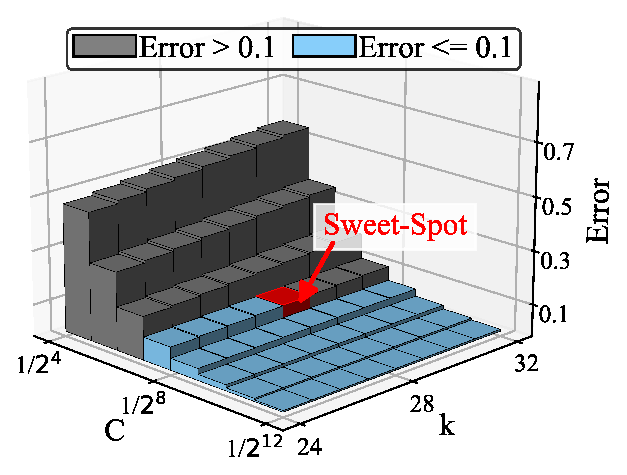
\includegraphics[width=\textwidth]{figs/OSDI/3d-fpr.eps}
         \caption{Error rate}
         \label{fig:hybrid}
     \end{subfigure}
     \hfill
     \begin{subfigure}[b]{0.23\textwidth}
         \centering
         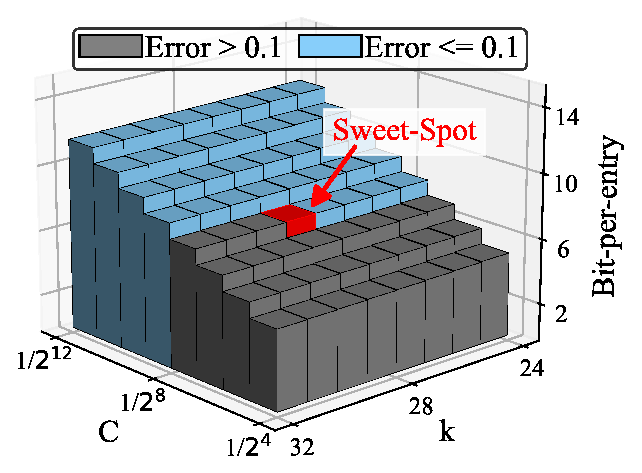
\includegraphics[width=\textwidth]{figs/OSDI/3d-bit.eps}
         \caption{Bit-per-entry}
         \label{fig:demand}
     \end{subfigure}
	 \vspace{-10pt}
	 \caption{\fixme{$\mathcal{E}_{FP}$ and memory requirements under varying C and k}}
	 \vspace{-10pt}
\label{fig:fp-CK}
\end{figure}

\FIG{fig:fp-CK} plots $\mathcal{E}_{FP}$ and
the number of bits per FP table entry (memory requirements) 
depending on $C$ and $k$. 
As expected, as $C$ gets lower, $\mathcal{E}_{FP}$ becomes smaller, but more
memory is needed.  Similarly, $\mathcal{E}_{FP}$
decreases as $k$ gets smaller. 
%This also results in high memory consumption. 
However, with smaller $k$,
\ours{} maintains a large number of small FP groups in the run.
Thus, the memory consumed by exact LBAs becomes significant,
which, in turn, increases bits per table entry.
\end{comment}

Eq.~(\ref{eq:fpr-relax}) tells us that $\mathcal{E}_{FP}$ is decided by
two variables $C$ and $k$. 
If our target error rate $\mathcal{E}_{FP}$ is 0.1, 
the best combination of <$C$, $k$>,
which requires the minimum memory,
is <0.0079, 28>. Using $|\FP{i}| = \ceil{log_{2}\frac{1}{C}}$,
each FP needs 7 bits to satisfy $C$ of 0.0079.
Since each FG group has 27 FP indices plus a 32-bit exact index,
the average size of the table entry is 7.89 bits.
Compared to typical exact indexing with 32-bit entries, \ours{} achieves 4.05$\times$ memory efficiency.
\begin{comment}
28개 일 경우 0.0079, 7, 27, (27*7+32)/32
29개 일 경우 0.
\end{comment}
%Even more, while exact indexing requires more bits to index data as an SSD capacity
%grows, \ours{} needs to increase an exact index. This means that \ours{} is a more scalable solution.

\begin{comment}
Eq.~(\ref{eq:fpr-relax}) cannot be solved for $FPR_{BF}$ using linear algebra.
However, it is clear that, for the same target FPR, $FPR_{BF}$ inbegin
Eq.~(\ref{eq:fpr-relax}) is higher than that in Eq.~(\ref{eq:fpr}).  If
$FPR_{T}^{R}$ is 0.1 and $n$=512, $FPR_{BF}$ from Eq.~(\ref{eq:fpr-relax}) is
4.2$\times$10$^{-4}$, which is higher than
2.06$\times$10$^{-4}$.  {The higher $FPR_{BF}$, the smaller $BF_i$} as
more false positive errors can be tolerated by \ours{}.  As a result, the relaxed BF needs
22-bit for each \BF{i}.
\FIXME{
가드를 고려하지 않고 수식을 정리했다는 언급이 필요함
}
\FIXME{
(n=512 --> $FPR_{BF}=0.00042065$ changed from 0.00041982, bit=12)
(n=28 --> $FPR_{BF}=0.00822996$, bit=7)
}
\end{comment}



\subsubsection{Lookup Optimization}
\label{sec:design:bf-lookup}

As discussed before, \ours{} has $O$($log\frac{n}{k}+k$) time to
look up an FP table.
To minimize lookup latency, we layout FPs in the memory to align with the
cache line boundary. Each FP group has 27 7-bit FPs, plus one exact index.
A 64B CPU cache line is large enough to accommodate two FP groups.
We split the cache line into two partitions -- 32B or 256-bit each -- and
place an FP group (221-bit) on each.  We increase $k$ from 27
to 32 so that each group fits in a 256-bit partition.  
It slightly increases the error rate $\mathcal{E}_{FP}$ (from 0.092 to 0.11), 
but we can better utilize the available memory.  
This memory layout also gets rid of extra memory references
caused by the miss-alignment.  
Moreover, since all the FPs are packed within a 64B integer,
comparing candidate FPs with an input LBA can be done at once
with few bit-wise operations.




%Looking up the table requires two steps: binary search and membership tests.
%The binary search over guards requires $O$($log~k$) time, where $k$ is the
%number of guards in the table.  The membership tests on candidate BFs between
%two guards require $O$(n) time. 
%As a result, \ours{} has
%logarithmic time complexity $O$($log~k+n$) for tree lookup. Thus, the
%majority of actual lookup time is spent on the membership test.  

%We minimize lookup latency by layouting BFs in the memory to align with the
%cache line boundary. Each guard embraces 28 7-bit BFs.
%The 64B CPU cache line is large enough to accommodate two guards and 56 BFs.
%Thus, we split the cache line into two partitions -- 32B or 256-bit each -- and
%place a guard and its BFs (228-bit in total) on each.  We increase $n$ from 28
%to 32 so that a guard plus its BFs fit in a 256-bit partition.  Even though it
%slightly increases the FPR (from 0.096 to 0.11), we can maximally
%utilize the available memory.  This memory layout also enables us to prefetch
%candidate BFs while performing binary search without any extra memory
%references.  Moreover, since all the BFs are packed within a 64B integer,
%comparing candidate BFs to an input LBA can be done at once
%with few bit-wise operations.



%The BF-based indexing is simple but gives us a huge benefit.  DFTL issues extra
%reads to fetch mapping entries from the flash when a cache miss happens.  In
%\ours{}, unnecessary reads occur only when BFs return false positive answers.
%However, 
%For \ours{} to outperform the demand-based FTLs, it should provide an acceptable
%FPR that is lower than a miss rate of them, while consuming less DRAM than
%the demand-based ones.  
%\ours{} also requires to perform binary search and scanning over BFs,
%which may cause lots of computation.  
%In \SEC{sec:opt:memory}, we explain various optimization techniques 
%to improve the accuracy of the BF-based indexing at low  
%memory usage and fast lookup latency in detail.
%Through various optimizations, \ours{}
%reduces the number of bits per BF to \JS{7.86} and provide the BF lookup
%latency of 0.55 $\mu$s.  The detailed explanation of the optimization is given
%in \SEC{sec:opt:memory}.

%In the worst case, all the BFs in a run should be examined (see
%\SEC{sec:opt:latency}).  We explain how these issues are addressed.






